\documentclass[landscape,fontscale=.8,paperwidth=24in,paperheight=18in]{baposter} % Adjust the font scale/size here


\usepackage{graphicx} % Required for including images
\graphicspath{{figures/}} % Directory in which figures are stored

\usepackage{amsmath} % For typesetting math
\usepackage{amssymb} % Adds new symbols to be used in math mode

\usepackage{booktabs} % Top and bottom rules for tables
\usepackage{enumitem} % Used to reduce itemize/enumerate spacing
\usepackage{palatino} % Use the Palatino font
\usepackage[font=small,labelfont=bf]{caption} % Required for specifying captions to tables and figures
\usepackage{listings} %for Java code


\usepackage{multicol} % Required for multiple columns
\setlength{\columnsep}{1.5em} % Slightly increase the space between columns
\setlength{\columnseprule}{0mm} % No horizontal rule between columns

\usepackage{tikz} % Required for flow chart
\usetikzlibrary{shapes,arrows} % Tikz libraries required for the flow chart in the template

\newcommand{\compresslist}{ % Define a command to reduce spacing within itemize/enumerate environments, this is used right after \begin{itemize} or \begin{enumerate}
\setlength{\itemsep}{1pt}
\setlength{\parskip}{0pt}
\setlength{\parsep}{0pt}
}

\definecolor{lightblue}{rgb}{0.145,0.6666,1} % Defines the color used for content box headers

\begin{document}

\begin{poster}
{
grid=false,
headerborder=closed, % Adds a border around the header of content boxes
colspacing=1em, % Column spacing
bgColorOne=white, % Background color for the gradient on the left side of the poster
bgColorTwo=white, % Background color for the gradient on the right side of the poster
borderColor=lightblue, % Border color
headerColorOne=white, % Background color for the header in the content boxes (left side)
headerColorTwo=white, % Background color for the header in the content boxes (right side)
headerFontColor=black, % Text color for the header text in the content boxes
boxColorOne=white, % Background color of the content boxes
textborder=roundedleft, % Format of the border around content boxes, can be: none, bars, coils, triangles, rectangle, rounded, roundedsmall, roundedright, roundedleft or faded
eyecatcher=false, % Set to false for ignoring the left logo in the title and move the title left
headerheight=0.1\textheight, % Height of the header
headershape=roundedright, % Specify the rounded corner in the content box headers, can be: rectangle, small-rounded, roundedright, roundedleft or rounded
headerfont=\Large\bf\textsc, % Large, bold and sans serif font in the headers of content boxes
%textfont={\setlength{\parindent}{1.5em}}, % Uncomment for paragraph indentation
columns =2,
linewidth=2pt % Width of the border lines around content boxes
}
%----------------------------------------------------------------------------------------
%	TITLE SECTION 
%----------------------------------------------------------------------------------------
%
{
\includegraphics[width=10em]{blank.png}} % First university/lab logo on the left
{\bf\textsc{RSA Encryption in Java via BigInteger and Simple Message Padding}}%vspace{0.5em}} % Poster title
{\textsc{ Chris and David Etler,  \hspace{12pt} Ocean County College}} % Author names and institution
{
\includegraphics[width=10em]{occ.png}} % Second university/lab logo on the right

%----------------------------------------------------------------------------------------
%	OBJECTIVES (0)
%----------------------------------------------------------------------------------------

\begin{posterbox}[name=objectives,column=0,row=0,span=13]{Objectives}

The objective of this project was to implement the RSA encryption scheme in Java. We provide the following deliverables to exhibit knowledge of RSA and public key cryptography:

\begin{enumerate}\compresslist
\item Generation of 4096-bit RSA keys
\item Encryption of integers less than 4096 bits in length via RSA
\item Conversion of plaintext to integer representation (\emph{padding scheme})
\item A graphical user interface for managing keys and encrypting messages in RSA.
\end{enumerate}

\vspace{0.3em} % When there are two boxes, some whitespace may need to be added if the one on the right has more content
\end{posterbox}

%----------------------------------------------------------------------------------------
%	INTRODUCTION (0)
%----------------------------------------------------------------------------------------

\begin{posterbox}[name=intro,column=0,below=objectives, span=13]{Introduction}

RSA cryptography is a industry-standard algorithm that implements public key cryptography in a simple yet extremely powerful way. Public key cryptography is a system which allows two parties to communicate by sharing one set of keys called \emph{public keys} and keeping another set called \emph{private keys} secret. This sort of system is highly useful everywhere from espionage to online gaming, as it allows clients to communicate openly without fear of any signal interception and without ever needing to communicate a shared secret over a private channel.

High level, the system works thus:
\begin{enumerate}
	\item Alice is trying to communicate with Bob secretly, while Eve is able to intercept any message that Alice sends to Bob or vice versa.
	\item In order to communicate with Bob, Alice needs to chose a shared secret with Bob which must be used to both verify Alice's identity and encode a message such that Eve will have no means of deciphering it without knowledge of the shared secret.
	\item Alice cannot communicate the shared secret openly with Bob, as there is no secure channel which Eve cannot overhear.
	\item Bob publishes a item that can encrypt a message in such a way that only he will ever be able to unlock it.
	\item This item is published freely such that both Alice and Eve have access to it. We can envision such a item as a padlock, which can be locked by anyone but only unlocked by one with the key.
	\item Alice can now write her message to Bob and lock it with the padlock. Only Bob will be able to unlock the padlock despite everyone having access to it.
	\item Alice also has her own padlock which can be used by Bob to send a message back to her.
\end{enumerate}

\begin{center}
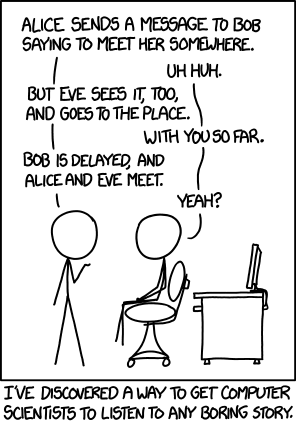
\includegraphics[width=.5\linewidth]{xkcd.png}
	\captionof*{figure}{Source: \emph{XKCD}}
\end{center}

\end{posterbox}

%----------------------------------------------------------------------------------------
%	RSA ALGORITHM (1)
%----------------------------------------------------------------------------------------

\begin{posterbox}[name=rsa,column=13,row=0,span=17]{RSA Algorithm} % This block's bottom aligns with the bottom of the conclusion block

There are a few technical considerations that must be taken into account to fully understand the workings of RSA. For one, we must develop a mathematical "padlock" in order to send messages abstractly rather than with physical padlocks. We will refer to these abstract padlocks as \emph{public keys} and the keys used to unlock them as \emph{private keys}, and both together as a \emph{key pair}. Key pairs must be generated algorithmically and keys must be complex enough such that the lock can't be "picked" by Eve.

The RSA algorithm works by generating two keys: a public and a private key. In reality, these keys are simply very long numbers. The security of the algorithm depends completely on the length of these numbers. In the past, numbers as low as 768-bit have been used, but modern practices call for no lower than 1024-bit; some implementations use as high as 4096-bit keys. For this implementation we decided to use 4096-bit keys, which would mean numbers on the order of $2^{4096}$.

The algorithm works as such:
\begin{enumerate}
	\item First, two prime numbers $p$ and $q$ are chosen. These two numbers together are used to form the public key. Specifically, the public key is ${pq = p * q}$. Both $p$ and $q$ should be of the same bit-length for security, so for a 4096-bit key, we chose to use two 2048-bit prime numbers. 
	\item A number $e$ is chosen and agreed upon by all using the algorithm. This is called the public exponent and the standard is $e = 65537$, though in practice any number mutually prime with ${(p-1)(q-1)}$ is usable. $65537$ is chosen as it's a prime number and is equal to ${2^{16}+1 = (1 \ll 16) + 1}$, which can be easily calculated by a computer.
	\item The private key $d$ is found by taking the \emph{modular inverse} of $e$ mod ${(p-1)*(q-1)}$. In our program, this number if found via the \emph{extended Euclidean algorithm}.
	\item A message is chosen and represented as an integer called $M$.
	\item From the message, a cypher-text $C$ is generated. $C = M^e\ mod\ pq$.
	\item The message is sent to the owner of the public key, who can decrypt the message using $M = C^d\ mod\ pq$.
\end{enumerate}

The algorithm derives strength from  a few different factors. First, it is very difficult to factor a large number into it's component primes. When a RSA public key is generated, two small prime numbers are generated separately and then multiplied by each-other to calculate the public key. It is easy for a computer to perform this task, taking mere seconds on even an antiquated laptop. However, such cannot be said about finding the two primes that make the public key given just the key itself. Even a modern supercomputer would be incapable of such a feat, even on the time-scale of years.

Further, RSA derives strength from how simple it is to calculate the modular inverse of $e$ mod $pq$ given just $(p-1)(q-1)$. This process is done via the extended Euclidean algorithm. The algorithm will always calculate the inverse of \verb|A| mod \verb|B| so long as one exists. The output are numbers $a$, $s$, and $t$ such that $a = GCD(A,B)$ and $A*s + B*t = a$. The second output, $s$, is the RSA decryption key when $A=e$ and ${B=(p-1)(q-1)}$. This can be calculated efficiently when $p$ and $q$ are originally known; however, finding this with only knowledge of the public key $pq$ is a monumental task, making RSA extremely secure. Code for the \emph{extended Euclidean}, as well as the RSA algorithm, is given to the right.
\end{posterbox}

%----------------------------------------------------------------------------------------

%----------------------------------------------------------------------------------------
%   HISTORY OF RSA (1)   
%----------------------------------------------------------------------------------------

\begin{posterbox}[name=history, column=13, below=rsa,span=17]{History}
\begin{multicols}{2}
RSA was first described publicly in 1977 by a trio of MIT mathematicians named Ron \textbf{R}ivest, Adi \textbf{S}hamir, and Leonard \textbf{A}dleman, after whom the algorithm is named. Prior to that the algorithm was used internally by the UK intelligence agency GCHQ, where it was discovered independently by Clifford Cocks. Despite having been discovered 4 years earlier, the algorithm is attributed to the MIT trio for their work being the first published for the general public.

Today, RSA is ubiquitous in many areas of security, mainly due to its simplicity and security. It is secure enough to be used by government espionage, yet simple enough to be implemented by amateurs. 

\begin{center}
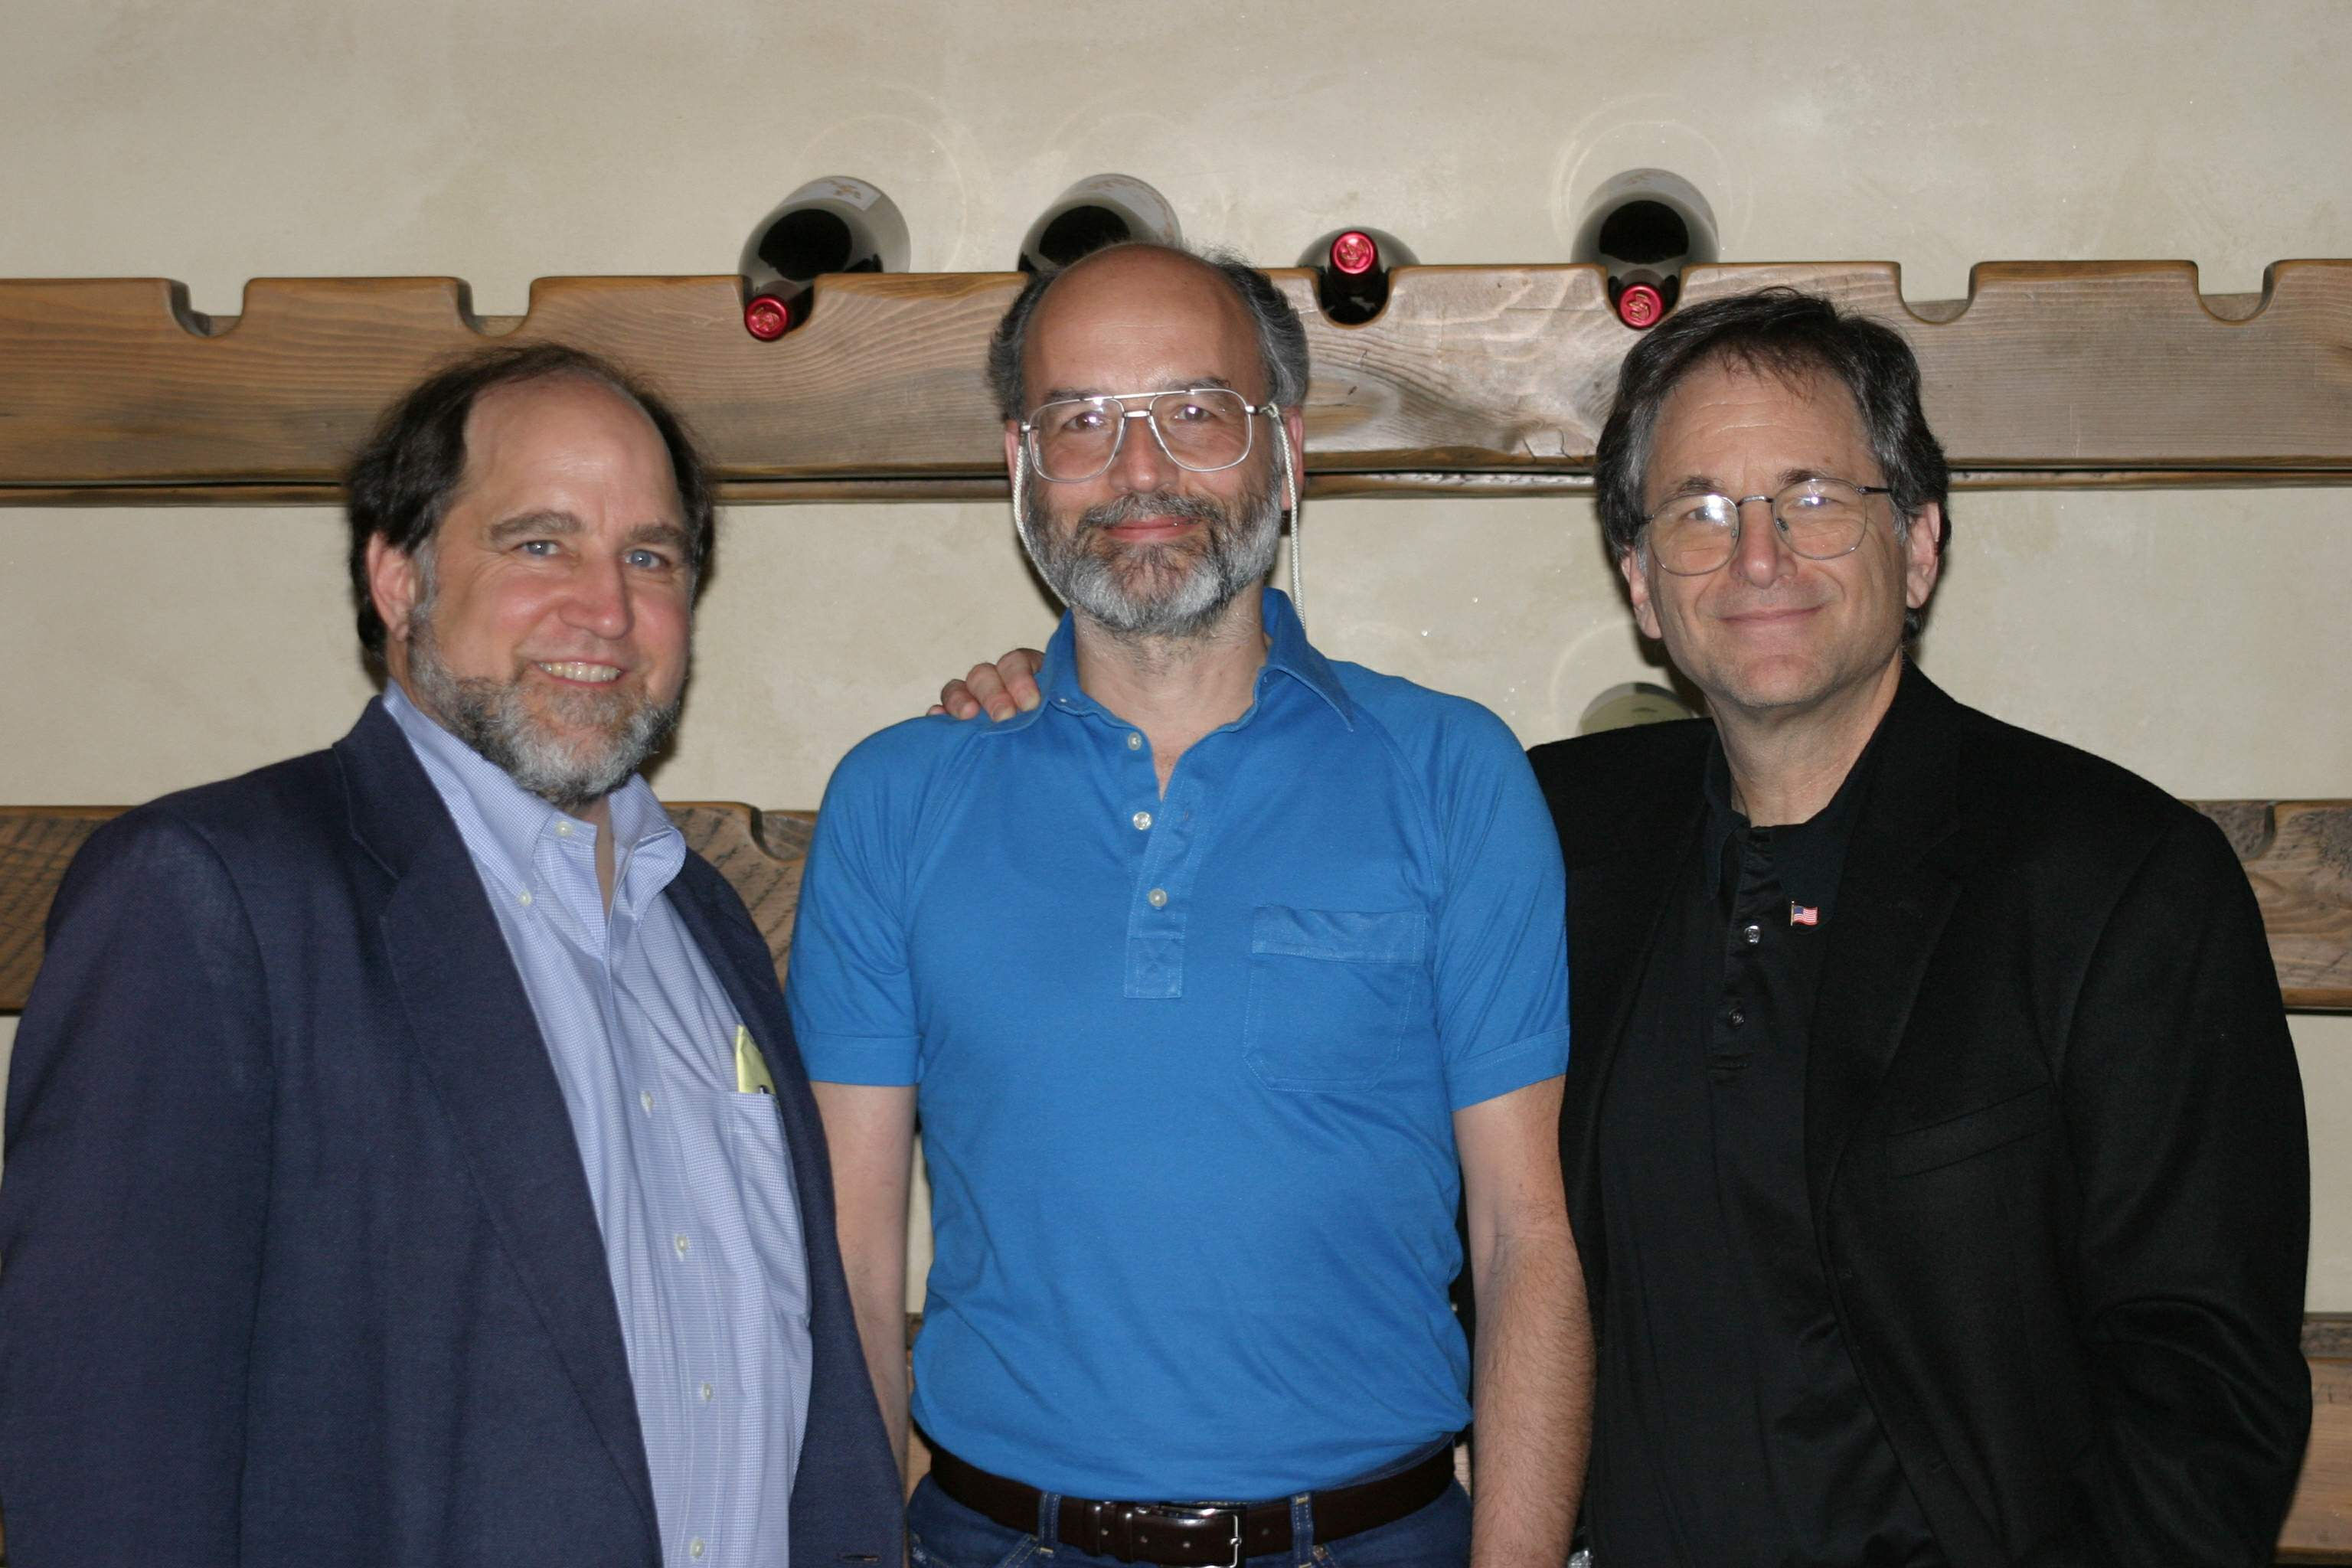
\includegraphics[width=1\linewidth]{RSA-2003.jpg}
	\captionof*{figure}{Ron Rivest, Adi Shamir, Len Adleman in 2003}
\end{center}
\end{multicols}
\end{posterbox}



%----------------------------------------------------------------------------------------
%	RSA ALGORITHM CODE (3)
%----------------------------------------------------------------------------------------

\begin{posterbox}[name=code,column=30,span=28,row=0]{RSA Algorithm Code (Excerpt)}

{\begin{verbatim}
public final class RSA {

    static final Message textConverter = new Message();

    public static BigInteger encrypt(String M, BigInteger e, BigInteger pq) {
        BigInteger Mn = textConverter.toInt(M);
        BigInteger C = M.modPow(e, pq);        
        return C;
    }
    public static BigInteger decrypt(String C, BigInteger d, BigInteger pq) {
        BigInteger Cn = textConverter.toInt(C);
        BigInteger M = C.modPow(d, pq);
        return M;
    }
    public static BigInteger[] generateKey() {
        Random rand = new Random();
        BigInteger p = BigInteger.probablePrime(2048, rand);
        BigInteger q = BigInteger.probablePrime(2048, rand);
        BigInteger[] key = {p.multiply(q), decryptionKey(p, q)};
        return key;
    }
    public static BigInteger decryptionKey(BigInteger p, BigInteger q) {
        BigInteger v = p.subtract(BigInteger.valueOf(1)).multiply(q.subtract(BigInteger.valueOf(1)));
        BigInteger d = Euclidean.extendedEuclidean(BigInteger.valueOf((1<<(1 << 4)) + 1), v)[1];
        if (d.compareTo(BigInteger.valueOf(0)) < 0) {
            d = d.add(v);
        }
        return d;
    }
}

public class Euclidean {
    public long[] extendedEuclidean(long A, long B) {
        long a = A, b = B, s = 1, t = 0;
        long u = 0, v = 1, r = 0, q = 0, nu, nv;
        while (b != 0) {
            r = a % b;
            q = (long) Math.floor(a / b);
            a = b;
            b = r;
            nu = s - u * q;
            nv = t - v * q;
            s = u;
            t = v;
            u = nu;
            v = nv;
        }
        long[] m = {a, s, t};
        return m;
    }
}
\end{verbatim}}

\end{posterbox}

%----------------------------------------------------------------------------------------



%----------------------------------------------------------------------------------------
%	CONCLUSION (2.0)
%----------------------------------------------------------------------------------------

\begin{posterbox}[name=conclusion, column=30, below=code, span=14]{Conclusion} 
This project served as great learning experience. Understanding and implementing the RSA algorithm is simple enough to be accessible to a student at a community college, yet ubiquitous and powerful enough to make a valuable chuck of knowledge. The implementation here is not complete, however. In practice a better padding scheme which adds entropy to the message is necessary to thwart attempts to decipher messages by accumulating a codex. Further, messaged signing by a second set of keys is common in practice to ensure that all messages were sent by the proper party. Any legitimate software application would be better off utilizing well-used RSA libraries which have been tested by many. However, for a hobby project, this program has been very useful to help understand the inner workings of the RSA algorithm.
\end{posterbox}


%----------------------------------------------------------------------------------------
%	MESSAGE PADDING (2.1)
%----------------------------------------------------------------------------------------

\begin{posterbox}[name=padding, column=44, below=code, span=14]{Message Padding}
In order to represent message plaintext as an integer for encryption, a \emph{padding scheme} was necessary. Our padding scheme encodes an symbol set of 100 characters as numbers between 00-99. A message is simply a series of these number combinations terminating with a single three-digit number that encodes the length of the message, so that leading zeros aren't lost.
\end{posterbox}



%----------------------------------------------------------------------------------------
%	ACKNOWLAGEMENTS (2.1)
%----------------------------------------------------------------------------------------

\begin{posterbox}[name=conclusion, column=44, below=padding, span=14]{Acknowledgments} 
We would like to thank Prof. Pezzimenti for his support in this project. We would also like to thanks as our parents for providing room and board while we conduct our studies. Further we would like to thanks Linus Torvalds for writing Git and the creators of NetBeans because they're seriously useful tools for development of applications in Java. Finally we'd like to thank Donald Knuth for writing \LaTeX and Brian Amberg for creating \verb|baposter|, the library through which this poster was rendered.
\end{posterbox}

\end{poster}

\end{document}